\chapter{Design}

\section{Overall System Design}

\subsection{Short description of the main parts of the system}

\subsection{System flowcharts showing an overview of the complete system}

\section{User Interface Designs}

\section{Hardwear Spesifiacation}

\section{Program Structure}

\subsection{Top-down design structure charts}

\subsection{Algorithms in pseudo-code for each data transformation process}

\subsection{Object Diagrams}

\subsection{Class Definitions}

\section{Prototyping}

\section{Definition of Data Requirements}

\subsection{Identification of all data input items}

\subsection{Identification of all data output items}

\subsection{Explanation of how data output items are generated}
Blank
\subsection{Data Dictionary}

\begin{tabular}{|p{1.5cm}|p{1.5cm}|l|l|l|p{2.5cm}|}
	\hline
	NAME & DATA TYPE & LENGTH & VALIDATION & EXAMPLE DATA & APPROXIMATE SIZE \\ \hline
	EventID & Integer & 0-9999 & Range & 10 & 4 Bytes \\ \hline
	CourseID & Integer & 0-9999 & Range & 10 & 4 Bytes \\ \hline
	Date & Date & DD/MM/YYYY & Range & 1 & 3 Bytes \\ \hline
	CircuitSeries & Boolean & 0 or 1 & Range & 1 & 2 Bytes \\ \hline
	Handicap10 & Boolean & 0 or 1 & Range & 1 & 2 Bytes \\ \hline
	Handicap25 & Boolean & 0 or 1 & Range & 1 & 2 Bytes \\ \hline
	HillClimb & Boolean & 0 or 1 & Range & 1 & 2 Bytes \\ \hline
	Transmedia & Boolean & 0 or 1 & Range & 1 & 2 Bytes \\ \hline
	Juvenile & Boolean & 0 or 1 & Range & 1 & 2 Bytes \\ \hline
	Code & String & 2 Characters & length & TR & 2 Bytes \\ \hline
	RiderID & Integer & 0-9999 & Range & 10 & 4 Bytes \\ \hline
	Forename & String & 50 Characters & length & Peter & 50 Bytes \\ \hline
	Surname & String & 50 Characters & length & Millard & 50 Bytes \\ \hline
	TCID & Integer & 0-9999 & Range & 10 & 4 Bytes \\ \hline
	Handicap10Points & Integer & 0-350 & Range & 125 & 4 Bytes \\ \hline
	CircuitPoints & Integer & 0-350 & Range & 125 & 4 Bytes \\ \hline
	TransmediaPoints & Integer & 0-350 & Range & 125 & 4 Bytes \\ \hline
	JuvenlePoints & Integer & 0-350 & Range & 125 & 4 Bytes \\ \hline
	CourseID & Integer & 0-9999 & Range & 10 & 4 Bytes \\ \hline
	RecordID & Integer & 0-9999 & Range & 10 & 4 Bytes \\ \hline
	RideTime & Time & HH:MM:SS & Range & 01:25:23 & 3 Bytes \\ \hline
	HandicapTime & Time & HH:MM:SS & Range & 00:25:23 & 3 Bytes \\ \hline
	RacePosition & Integer & 1-50 & Range & 05 & 4 Bytes \\ \hline
	Club & String & 50 Characters & Length & Team Cambridge & 100 Bytes \\ \hline
	Age & Integer & 12 – 99 & Range & 18 & 4 Bytes \\ \hline
\end{tabular}

\subsection{Identification of appropriate storage media}

\section{Database Design}

\subsection{Normalisation}

\subsubsection{ER Diagrams}
\begin{figure}[H]
    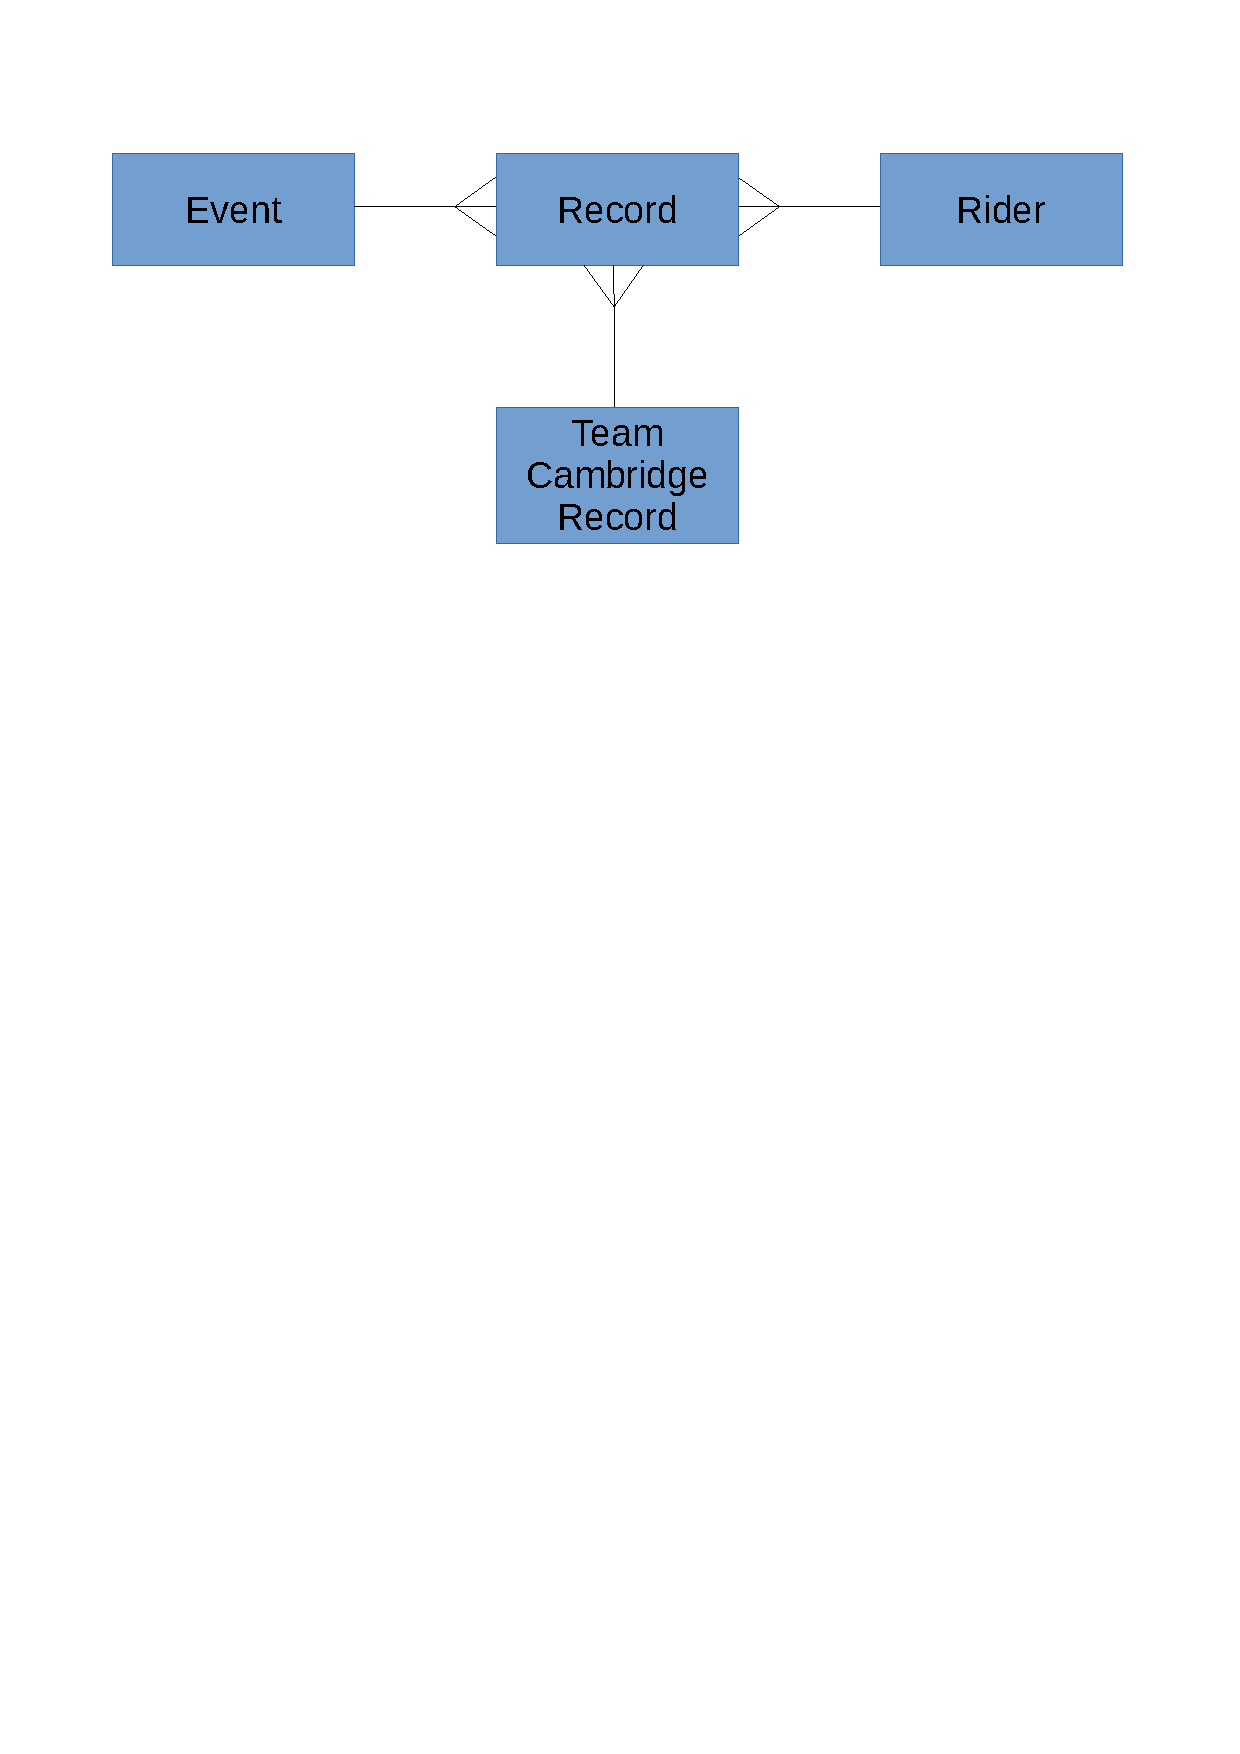
\includegraphics[width=\textwidth]{./ER/ERDesing.pdf}
\end{figure}

\subsubsection{Entity Descriptions}

Event(\underline{EventID}, \emph{CourseID} , \emph{EventTypeID}, Date )

Course(\underline{CourseID}, CourseCode, CourseDistance)

Event Referance(\underline{EventReferanceID}, \emph{EventID}, \emph{EventTypeID})

Event Type(\underline{EventTypeID}, EventType)

Rider(\underline{RiderID}, Forename, Surname)

Club Reference(\underline{ClubReferance}, \emph{RiderID}, \emph{ClubID}, DateJoined, DateLeft)

Club(\underline{ClubID}, Club)

Record(\underline{RecordID}, \emph{EventID}, RdieTime, Age, HandicapMod)

Event Points(\underline{EventPointsID}, \emph{RecordID}, EventPointsType, EventPoints)

\subsubsection{UNF to 3NF}
\underline{UNF}


\begin{tabular}{l l l}
EventID        & Age              & Date               \\
EventPoints    & EventType        & EventPointType     \\
ClubReferance  & RiderID          & Forename           \\
Surname        & HandicapMod      & EventPointsID      \\
Club           & RecordID         & RideTime           \\
CourceID       & CourceCode       & CourceDistance     \\
DateJoined     & DateLeft         & EventReferanceID   \\
EventTypeID    & ClubID           &                    \\

\end{tabular}

\underline{1NF}

\begin{tabular}{|l l|l|}
\hline
REPEATING           &                 & NON-REPEATING       \\ \hline
\underline{RecordID}& RideTime        & \underline{EventID} \\ \hline
\underline{EventID} & EventPointsType & Date                \\ \hline
ClubReferance       & DateLeft        & CourseID            \\ \hline
Surname             & HandicapMod     & CourseCode          \\ \hline
DateJoined          & RiderID         & CorseDistance       \\ \hline 
EventPointsID       & Age             & EventReferanceID    \\ \hline
EventTypeID         & ClubID          &                     \\ \hline
\end{tabular}




\underline{2NF}

\begin{tabular}{|l|l|}
\hline
\underline{RecordID}  & \underline{EventID} \\ \hline
Forename             & Date                \\ \hline
Surname              & CourceID            \\ \hline
ClubReferance        & CourceCode          \\ \hline
Club                 & CourceDistance      \\ \hline
DateJoined           & EventTypeID         \\ \hline
DateLeft             & EventType           \\ \hline
ClubID               & EventReferanceID    \\ \hline
                     &                     \\ \hline
\underline{RecordID} &                     \\ \hline
\underline{EventID}  &                     \\ \hline 
EventPointsID        &                     \\ \hline
RideTIme             &                     \\ \hline
Age                  &                     \\ \hline
HandicapMod          &                     \\ \hline
EventPoints          &                     \\ \hline
EventPointsType      &                     \\ \hline
\end{tabular}

\underline{3NF}

\begin{tabular}{|l|l|l|l|}
\hline
\begin{tabular}{l}
	\\
	\underline{EventID} \\
	\emph{CourseID}     \\
	Date                \\
	\\
\end{tabular}& \begin{tabular}{l}
	\underline{CourseID} \\
	CourseCode           \\
	CourseDistance       \\
\end{tabular} & \begin{tabular}{l}
	\underline{EventReferanceID} \\
	\emph{EventID}               \\
	\emph{EventTypeID}           \\
\end{tabular} &\begin{tabular}{l}
	\underline{RiderID} \\
	Forename            \\
	Surname             \\
\end{tabular} \\ \hline
\begin{tabular}{l}
	\underline{ClubReference} \\
	\emph{RiderID}            \\
	\emph{ClubID}             \\
	DateJoined                \\
	DateLeft                  \\
\end{tabular} & \begin{tabular}{l}
	\\
	\underline{RecordID} \\
	\emph{EventID}       \\
	\emph{RiderID }      \\
	RideTime             \\
	Age                  \\
	HandicapMod          \\
	\\
\end{tabular} & \begin{tabular}{l}
	\underline{EventPointsID} \\
	\emph{RecordID}           \\
	EventPointsType           \\
	EventPoints               \\
\end{tabular} & \begin{tabular}{l}
	\underline{ClubID} \\
	Club               \\
\end{tabular} \\ \hline
\begin{tabular}{l}
	\\
	\underline{EventTypeID} \\
	EventType               \\
	\\
\end{tabular} & & & \\ \hline 
\end{tabular}

\section{Security and Integrity of the System and Data}

\subsection{Security and Integrity of Data}

\subsection{System Security}

\section{Validation}

\section{Testing}

\begin{landscape}
\subsection{Outline Plan}

\begin{center}
    \begin{tabular}{|p{2cm}|p{5cm}|p{5cm}|p{4cm}|}
        \hline
        \textbf{Test Series} & \textbf{Purpose of Test Series} & \textbf{Testing Strategy} & \textbf{Strategy Rationale}\\ \hline
        Example & Example & Example & Example \\ \hline
    \end{tabular}
\end{center}

\subsection{Detailed Plan}

\begin{center}
    \begin{longtable}{|p{1.5cm}|p{2.5cm}|p{2.5cm}|p{2cm}|p{2cm}|p{2cm}|p{2cm}|p{2cm}|}
        \hline
        \textbf{Test Series} & \textbf{Purpose of Test} & \textbf{Test Description} & \textbf{Test Data} & \textbf{Test Data Type (Normal/ Erroneous/ Boundary)} & \textbf{Expected Result} & \textbf{Actual Result} & \textbf{Evidence}\\ \hline
        Example & Example & Example & Example & Example & Example & Example & Example \\ \hline
    \end{longtable}
\end{center}
\end{landscape}
